%%%%%%%%%%%%%%%%%%%%%%%%%%%%%%%%%%%%%%%%%%%%%%%%%%%%%%%%%%%%%%%%%%%%%%%%%%%%%%%
%                                                                             %
% 04 - Acerca de                                                              %
%                                                                             %
%%%%%%%%%%%%%%%%%%%%%%%%%%%%%%%%%%%%%%%%%%%%%%%%%%%%%%%%%%%%%%%%%%%%%%%%%%%%%%%
\chapter{\textcolor{azulescom}{Acerca de}}

\section{¿Qué es el proyecto?}
En esta sección se puede leer una introducción a \textit{SkyPrice}, destacando
que forma parte de un proyecto de titulación para la carrera de Ingeniería en
Sistemas Computacionales del Instituto Politécnico Nacional. En la figura
\ref{fig:intro} se muestra la sección en cuestión en la página.

\begin{figure}[H]
  \centering
  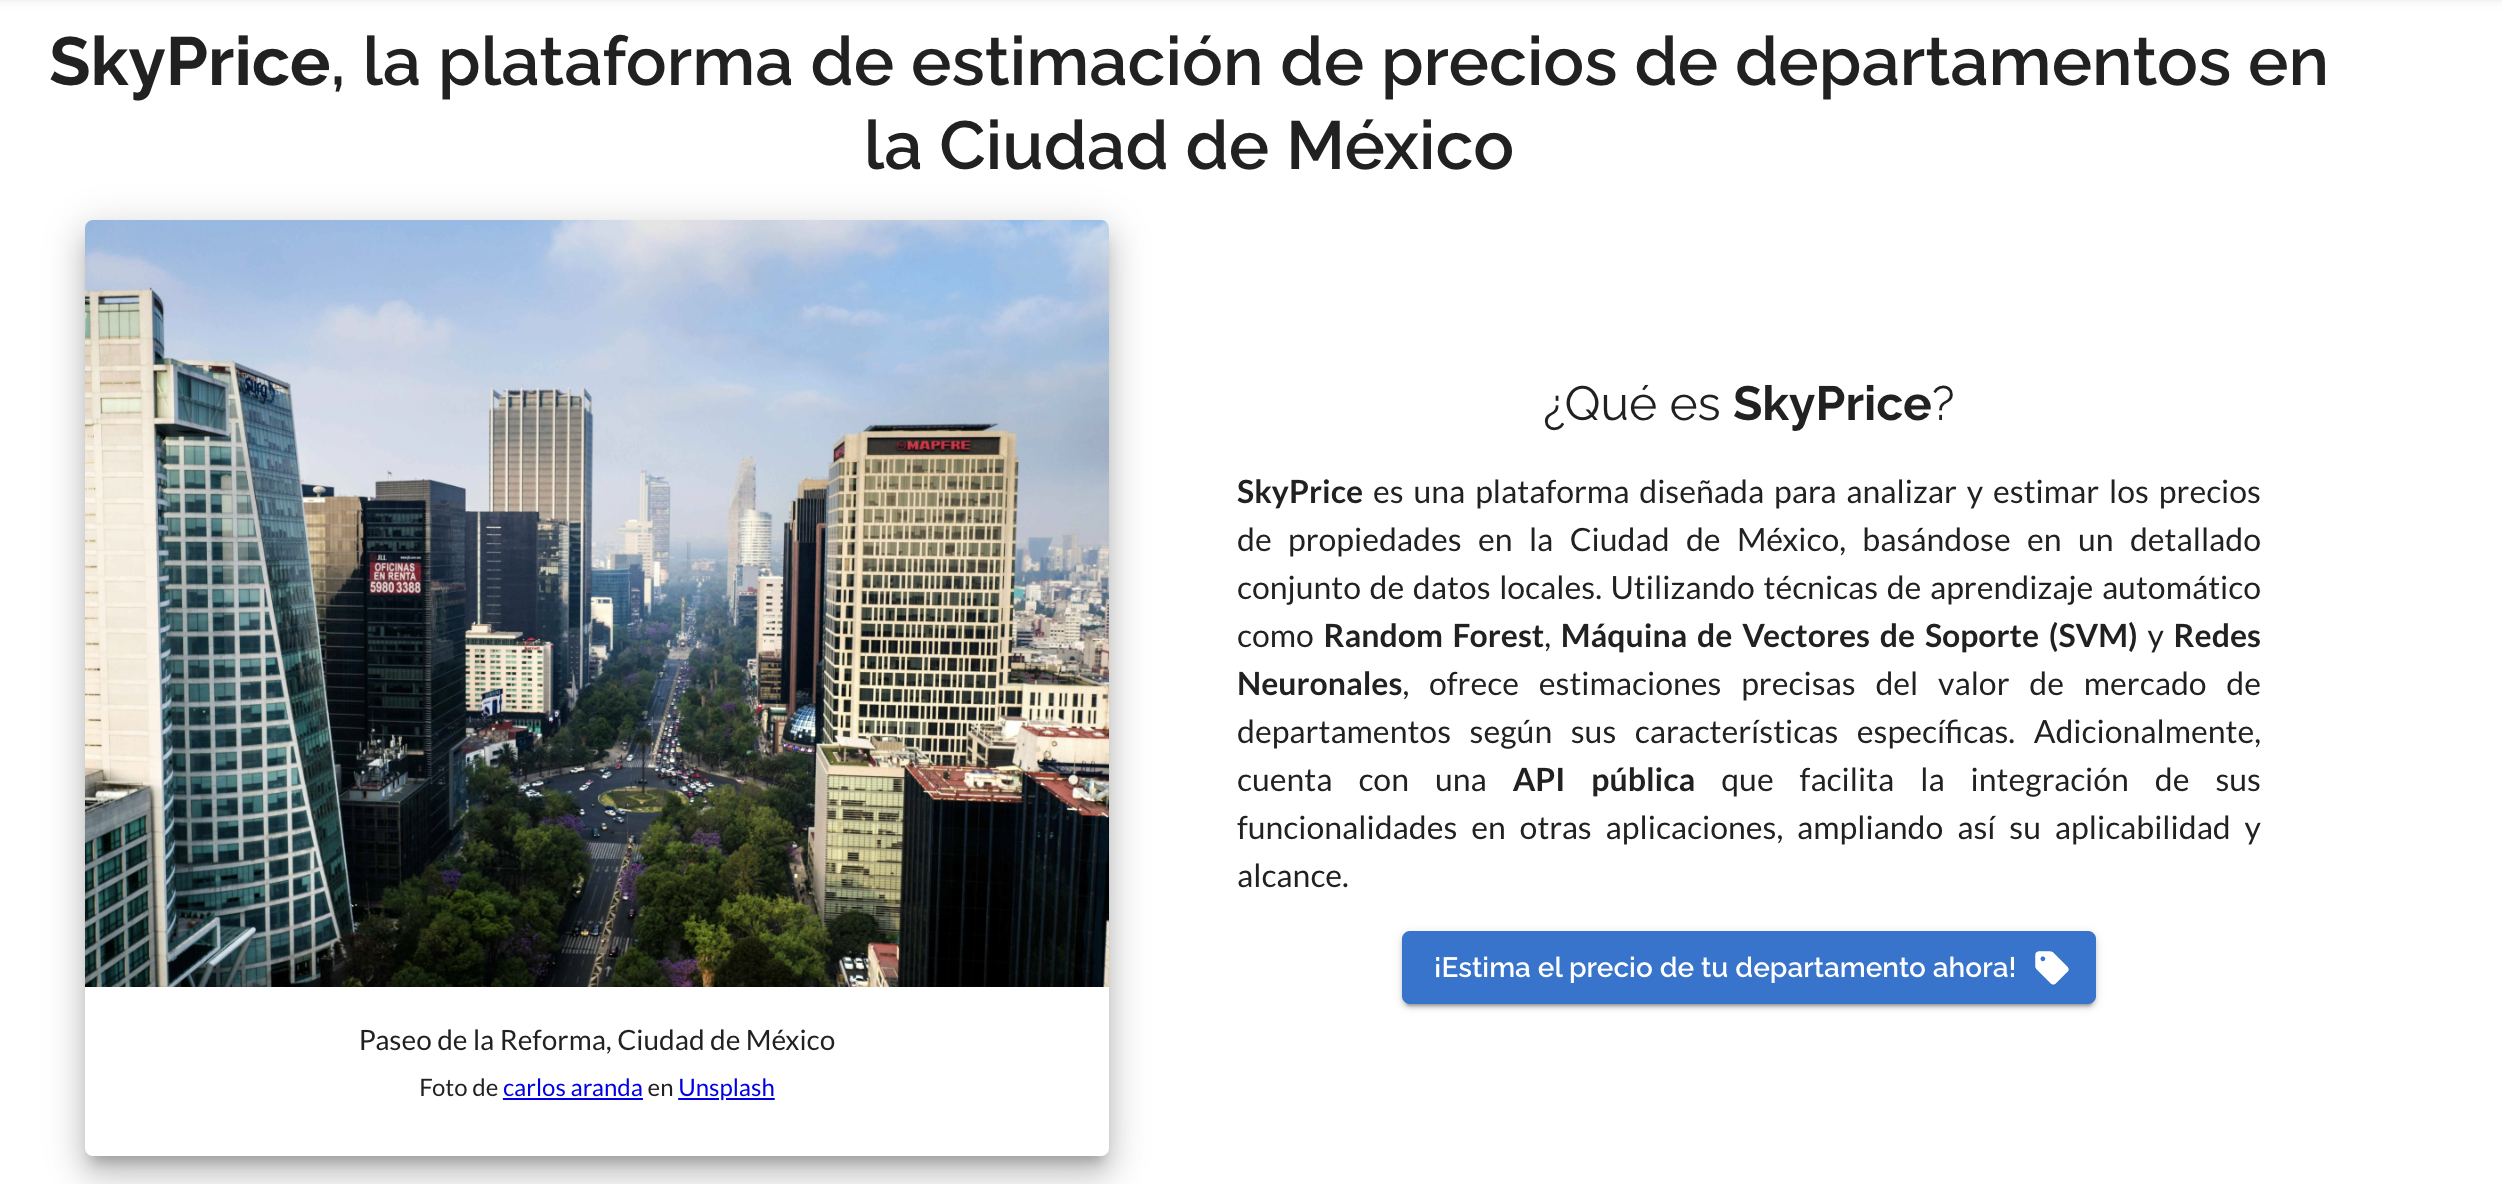
\includegraphics[width=0.8\textwidth]{imagenes/04-acerca-de/intro.png}
  \caption{Sección de introducción en la página de Acerca de.}
  \label{fig:intro}
\end{figure}

\section{Datos}
La sección de datos comienza con una breve explicación de los datos recabados
para realizar el entrenamiento de los modelos, así como la fuente y método de
limpieza y procesamiento de los mismos. En la figura \ref{fig:datos} se muestra
la sección en cuestión en la página.

\begin{figure}[H]
  \centering
  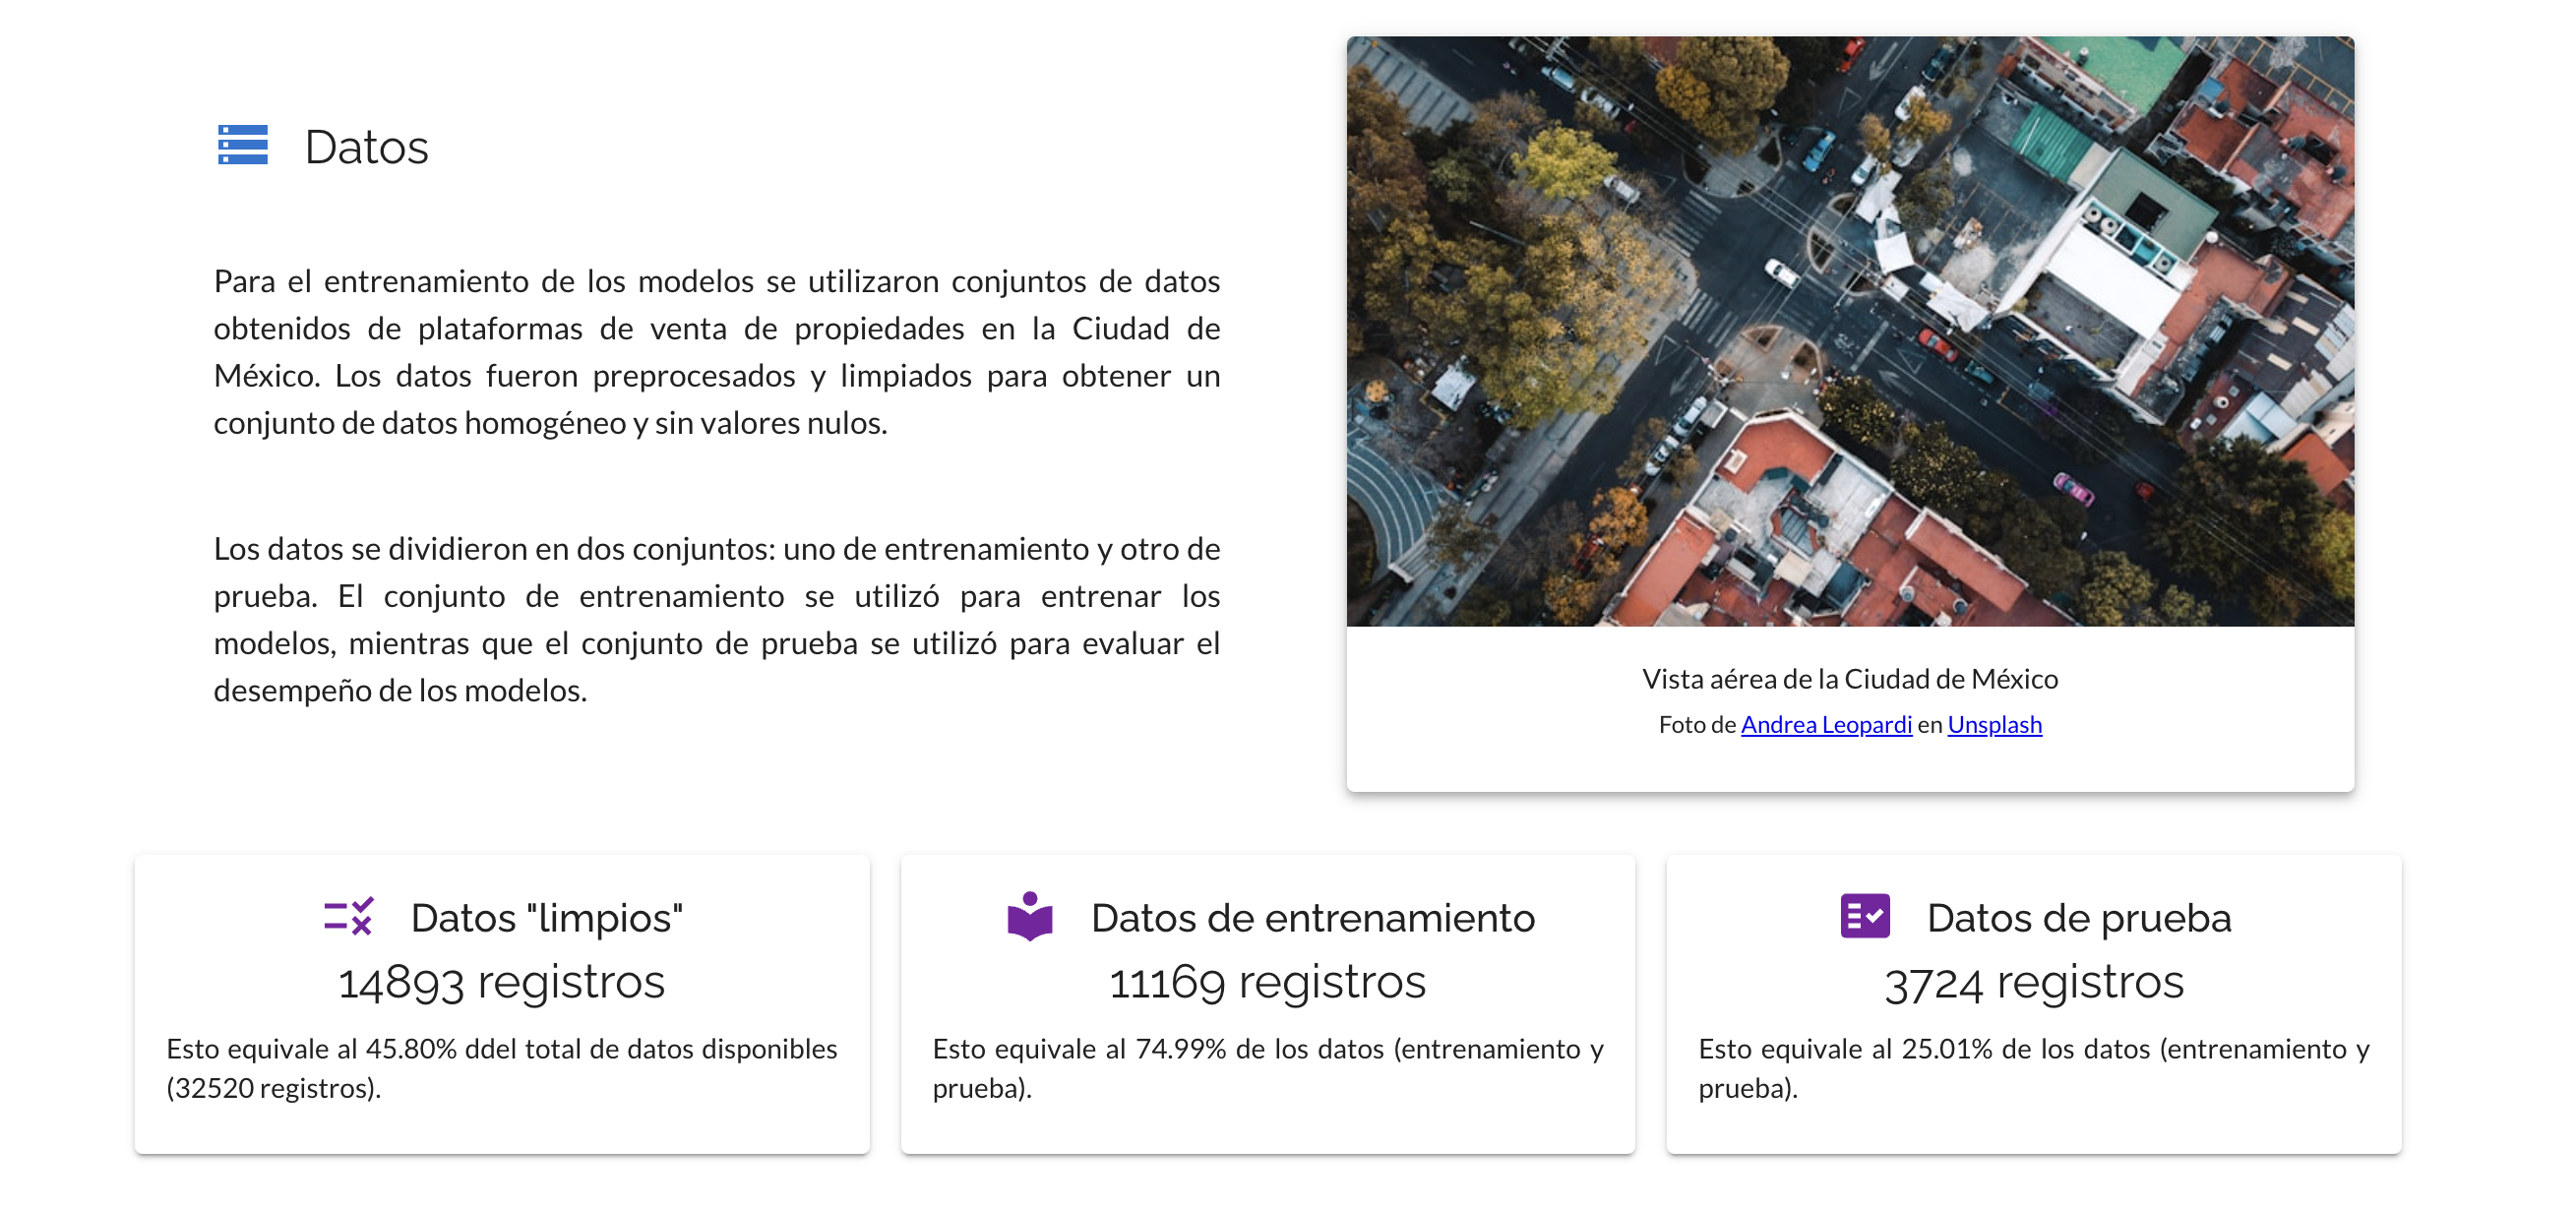
\includegraphics[width=0.8\textwidth]{imagenes/04-acerca-de/datos.png}
  \caption{Sección de datos en la página de Acerca de.}
  \label{fig:datos}
\end{figure}

\subsection{Mapa interactivo}
En la sección de datos también se incluye una tarjeta con información del mapa
interactivo, en la cual se muestra una imagen del mapa y se explica cómo
funciona. En la figura \ref{fig:mapa} se muestra la sección en cuestión en la
página.

\begin{figure}[H]
  \centering
  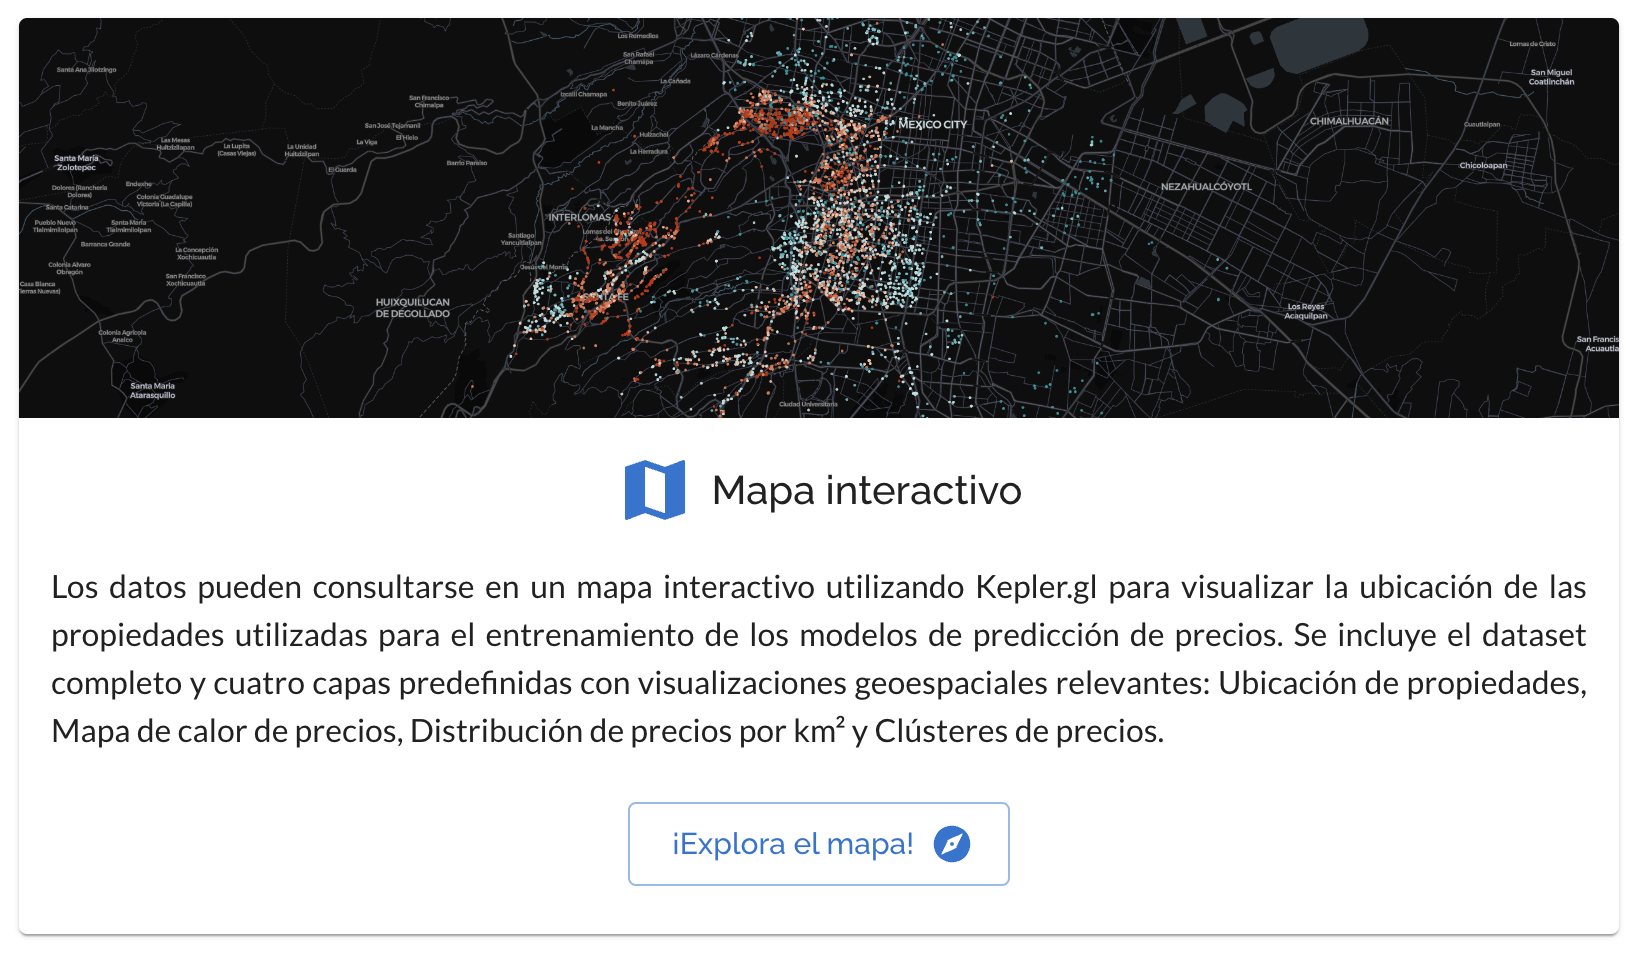
\includegraphics[width=0.8\textwidth]{imagenes/04-acerca-de/mapa.png}
  \caption{Sección de mapa interactivo en la página de Acerca de.}
  \label{fig:mapa}
\end{figure}

\section{Modelos}
La sección de modelos tiene como objetivo comunicar la metodología y detalles
de los modelos de aprendizaje automático utilizados en el proyecto. En la figura
\ref{fig:modelos} se muestra la sección en cuestión en la página.

\begin{figure}[H]
  \centering
  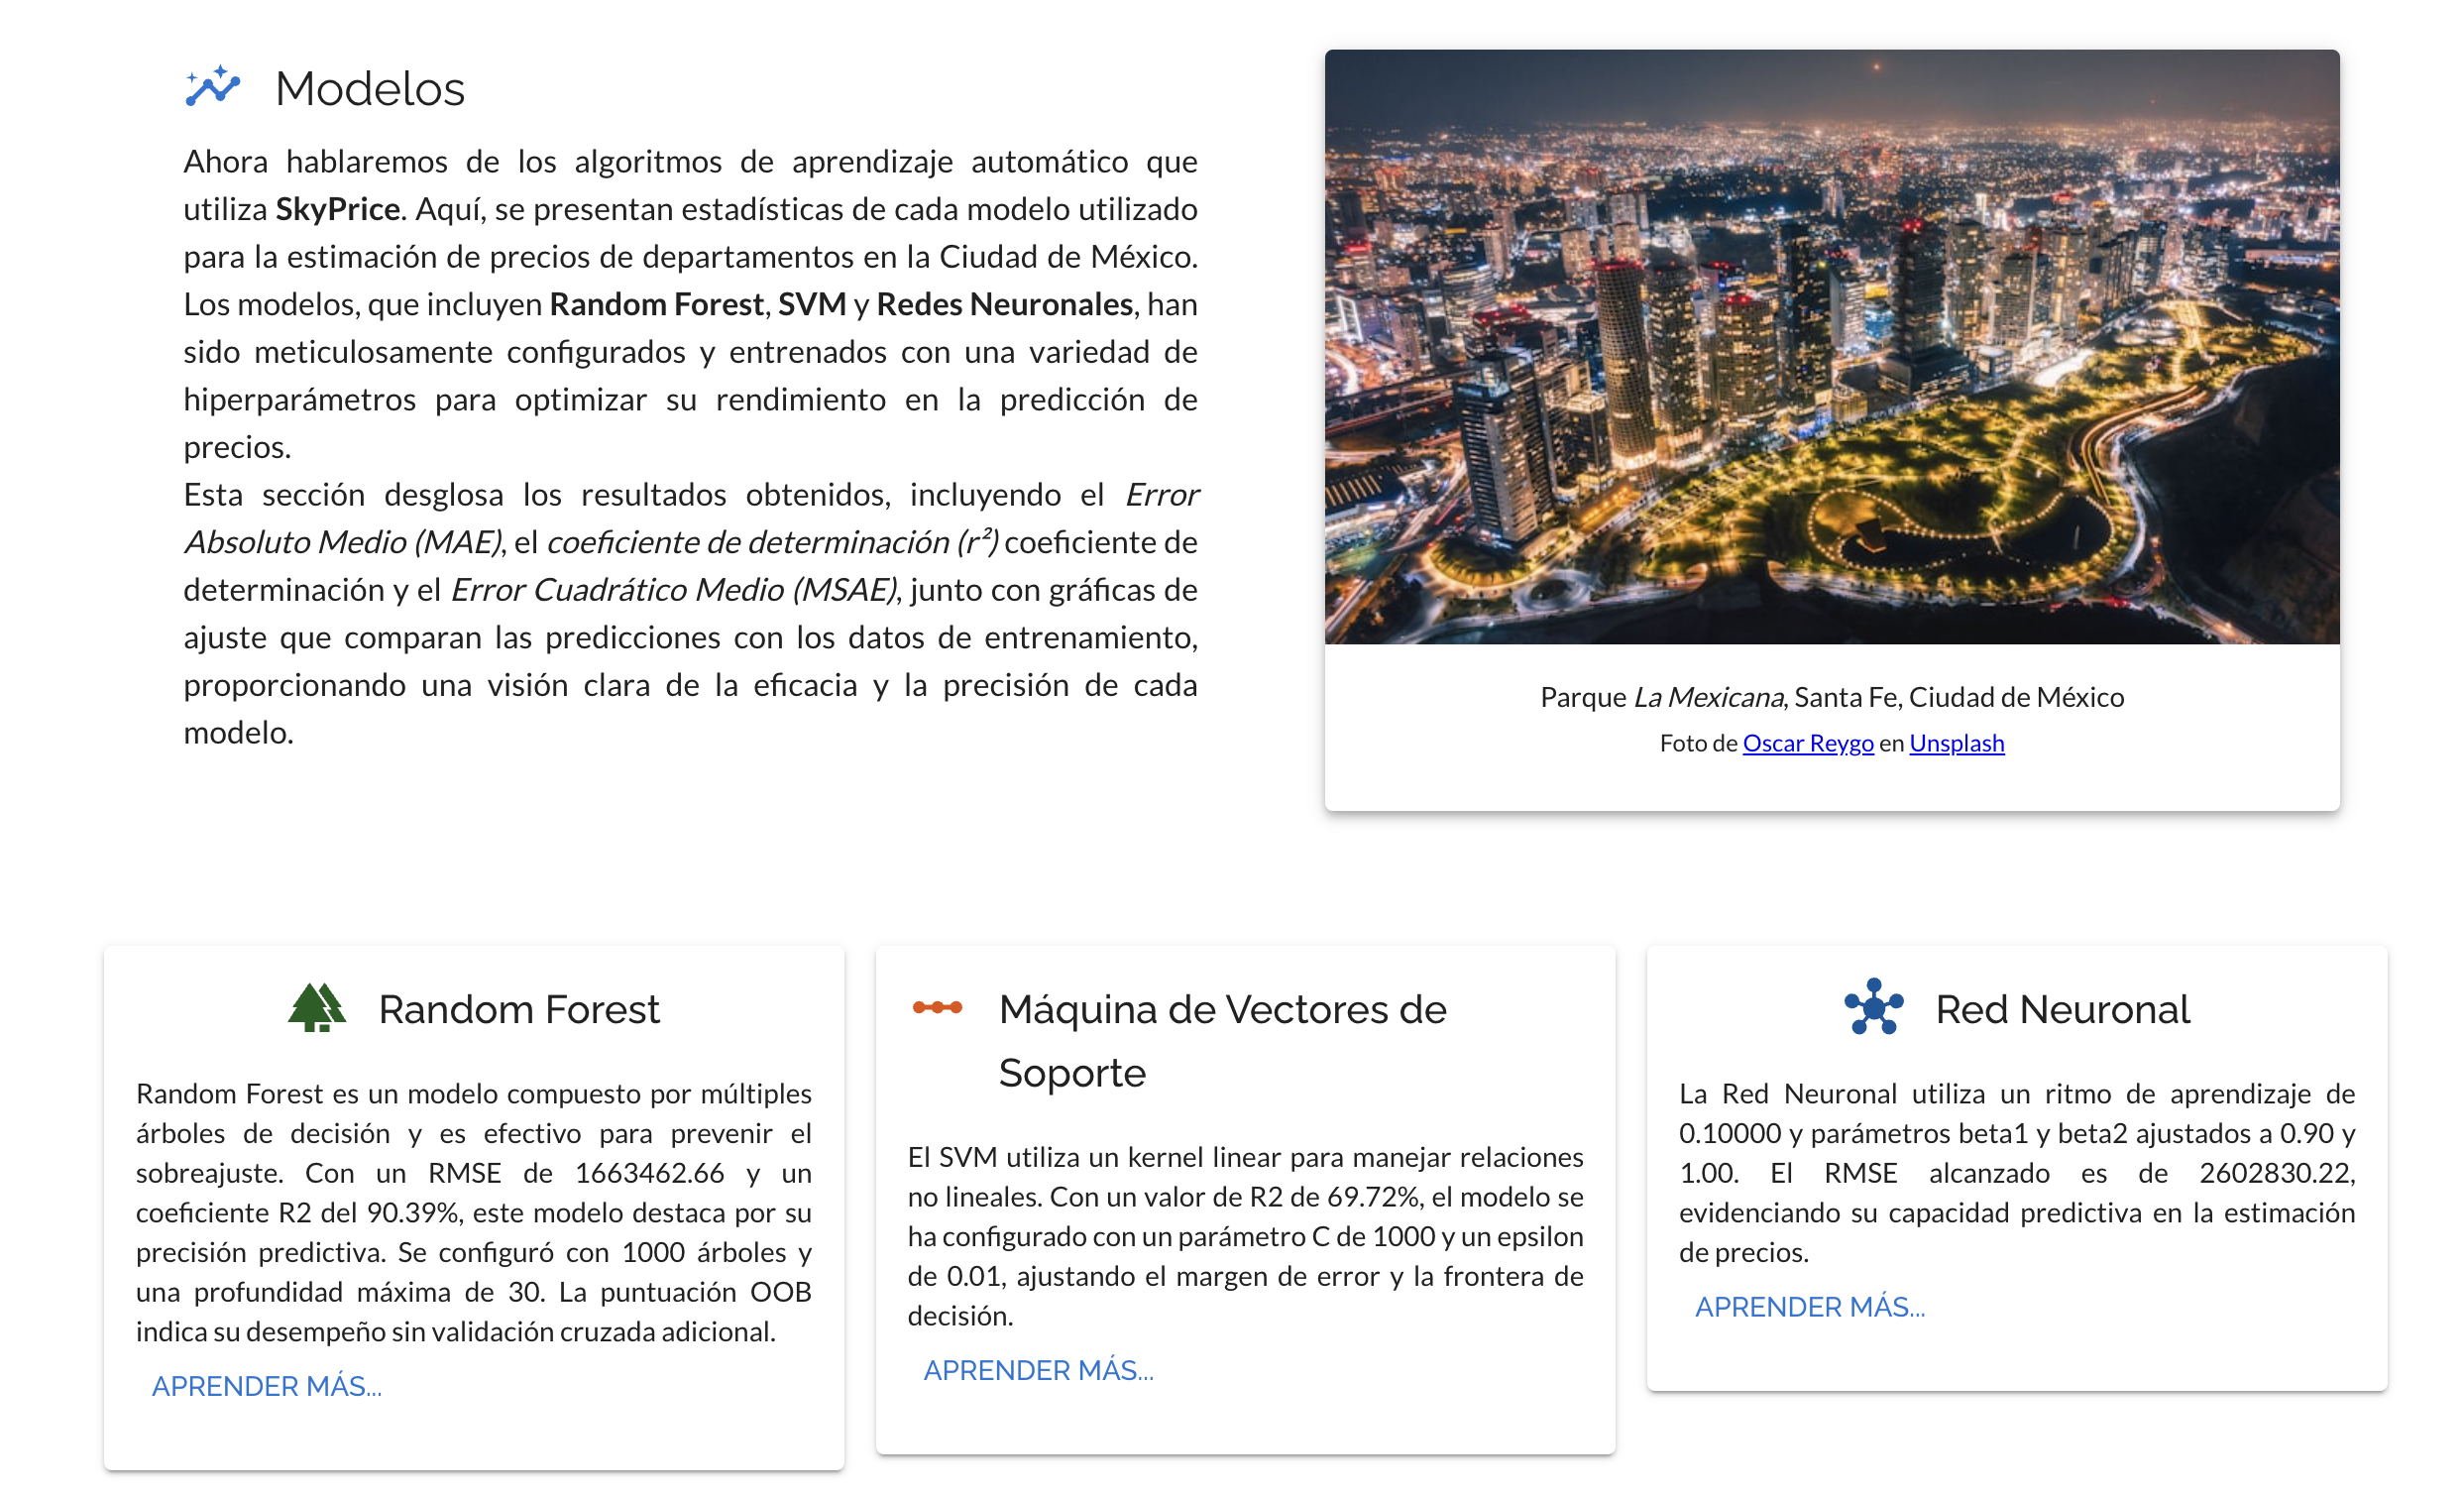
\includegraphics[width=0.8\textwidth]{imagenes/04-acerca-de/modelos.png}
  \caption{Sección de modelos en la página de Acerca de.}
  \label{fig:modelos}
\end{figure}

\subsection{Gráfica de ajuste}
En la sección de modelos también se incluye una gráfica de ajuste, en la cual se
muestra la predicción de los precios de los vuelos en comparación con los precios
reales. En la figura \ref{fig:ajuste} se muestra la sección en cuestión en la
página.

\begin{figure}[H]
  \centering
  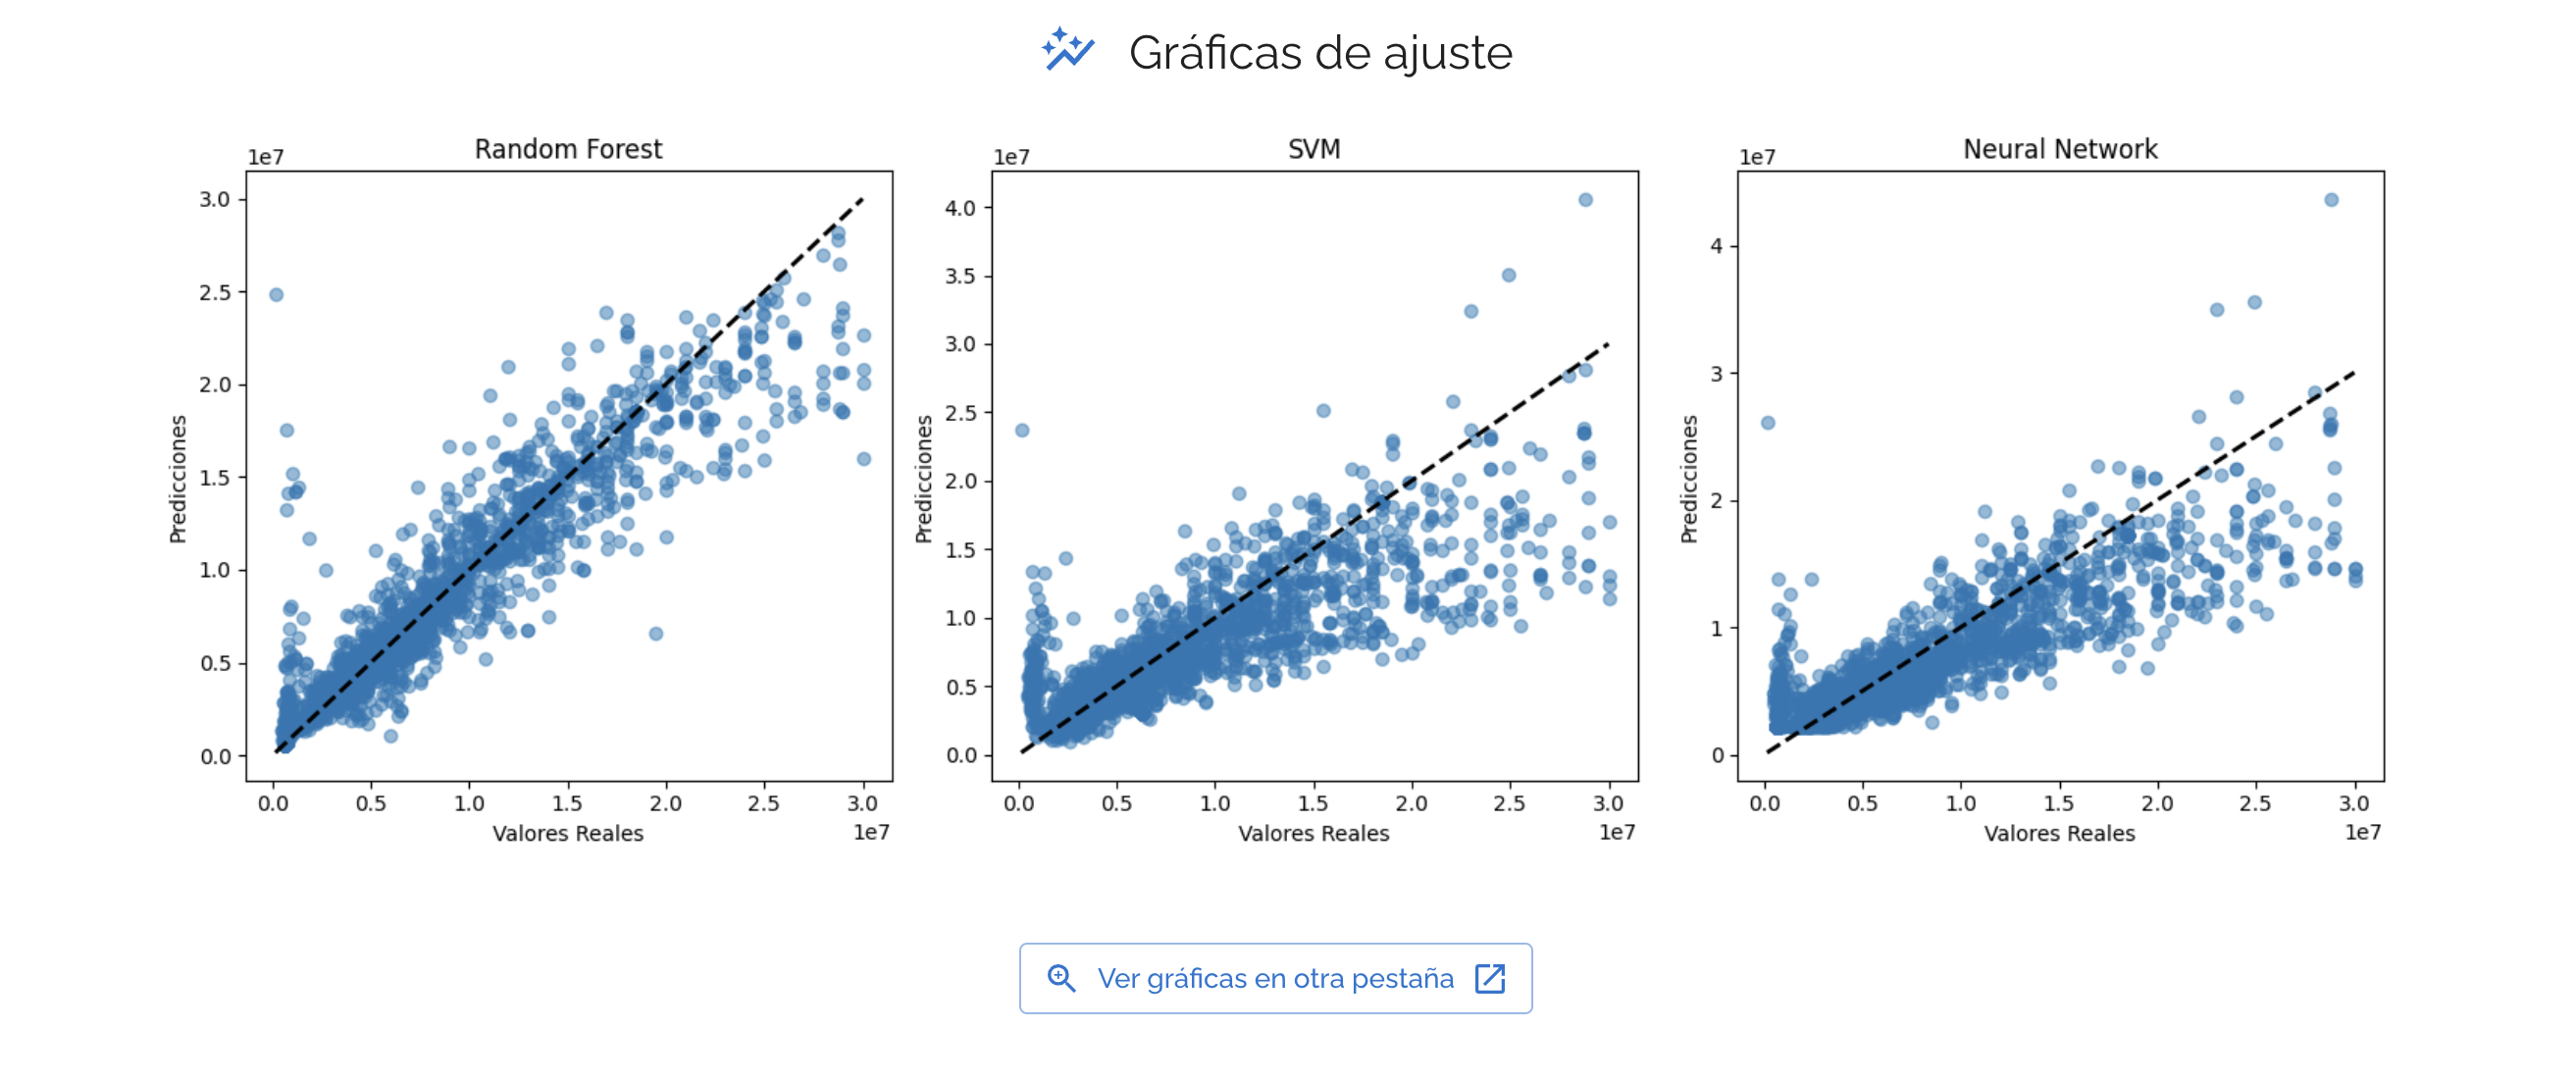
\includegraphics[width=0.8\textwidth]{imagenes/04-acerca-de/graficas-ajuste.png}
  \caption{Gráfica de ajuste en la página de Acerca de.}
  \label{fig:ajuste}
\end{figure}

Se incluye un botón para \textit{Ver gráficas en otra pestaña}, el cual permite
que el navegador incorpore elementos de interactividad en la gráfica, como
acercar, alejar, descargar, entre otros.

\subsection{Gráfica de métricas}
En la sección de modelos también se incluye una gráfica de métricas, en la cual
se muestra una comprativa de distintas métricas de los modelos utilizados. En la
figura \ref{fig:metricas} se muestra la sección en cuestión en la página.

\begin{figure}[H]
  \centering
  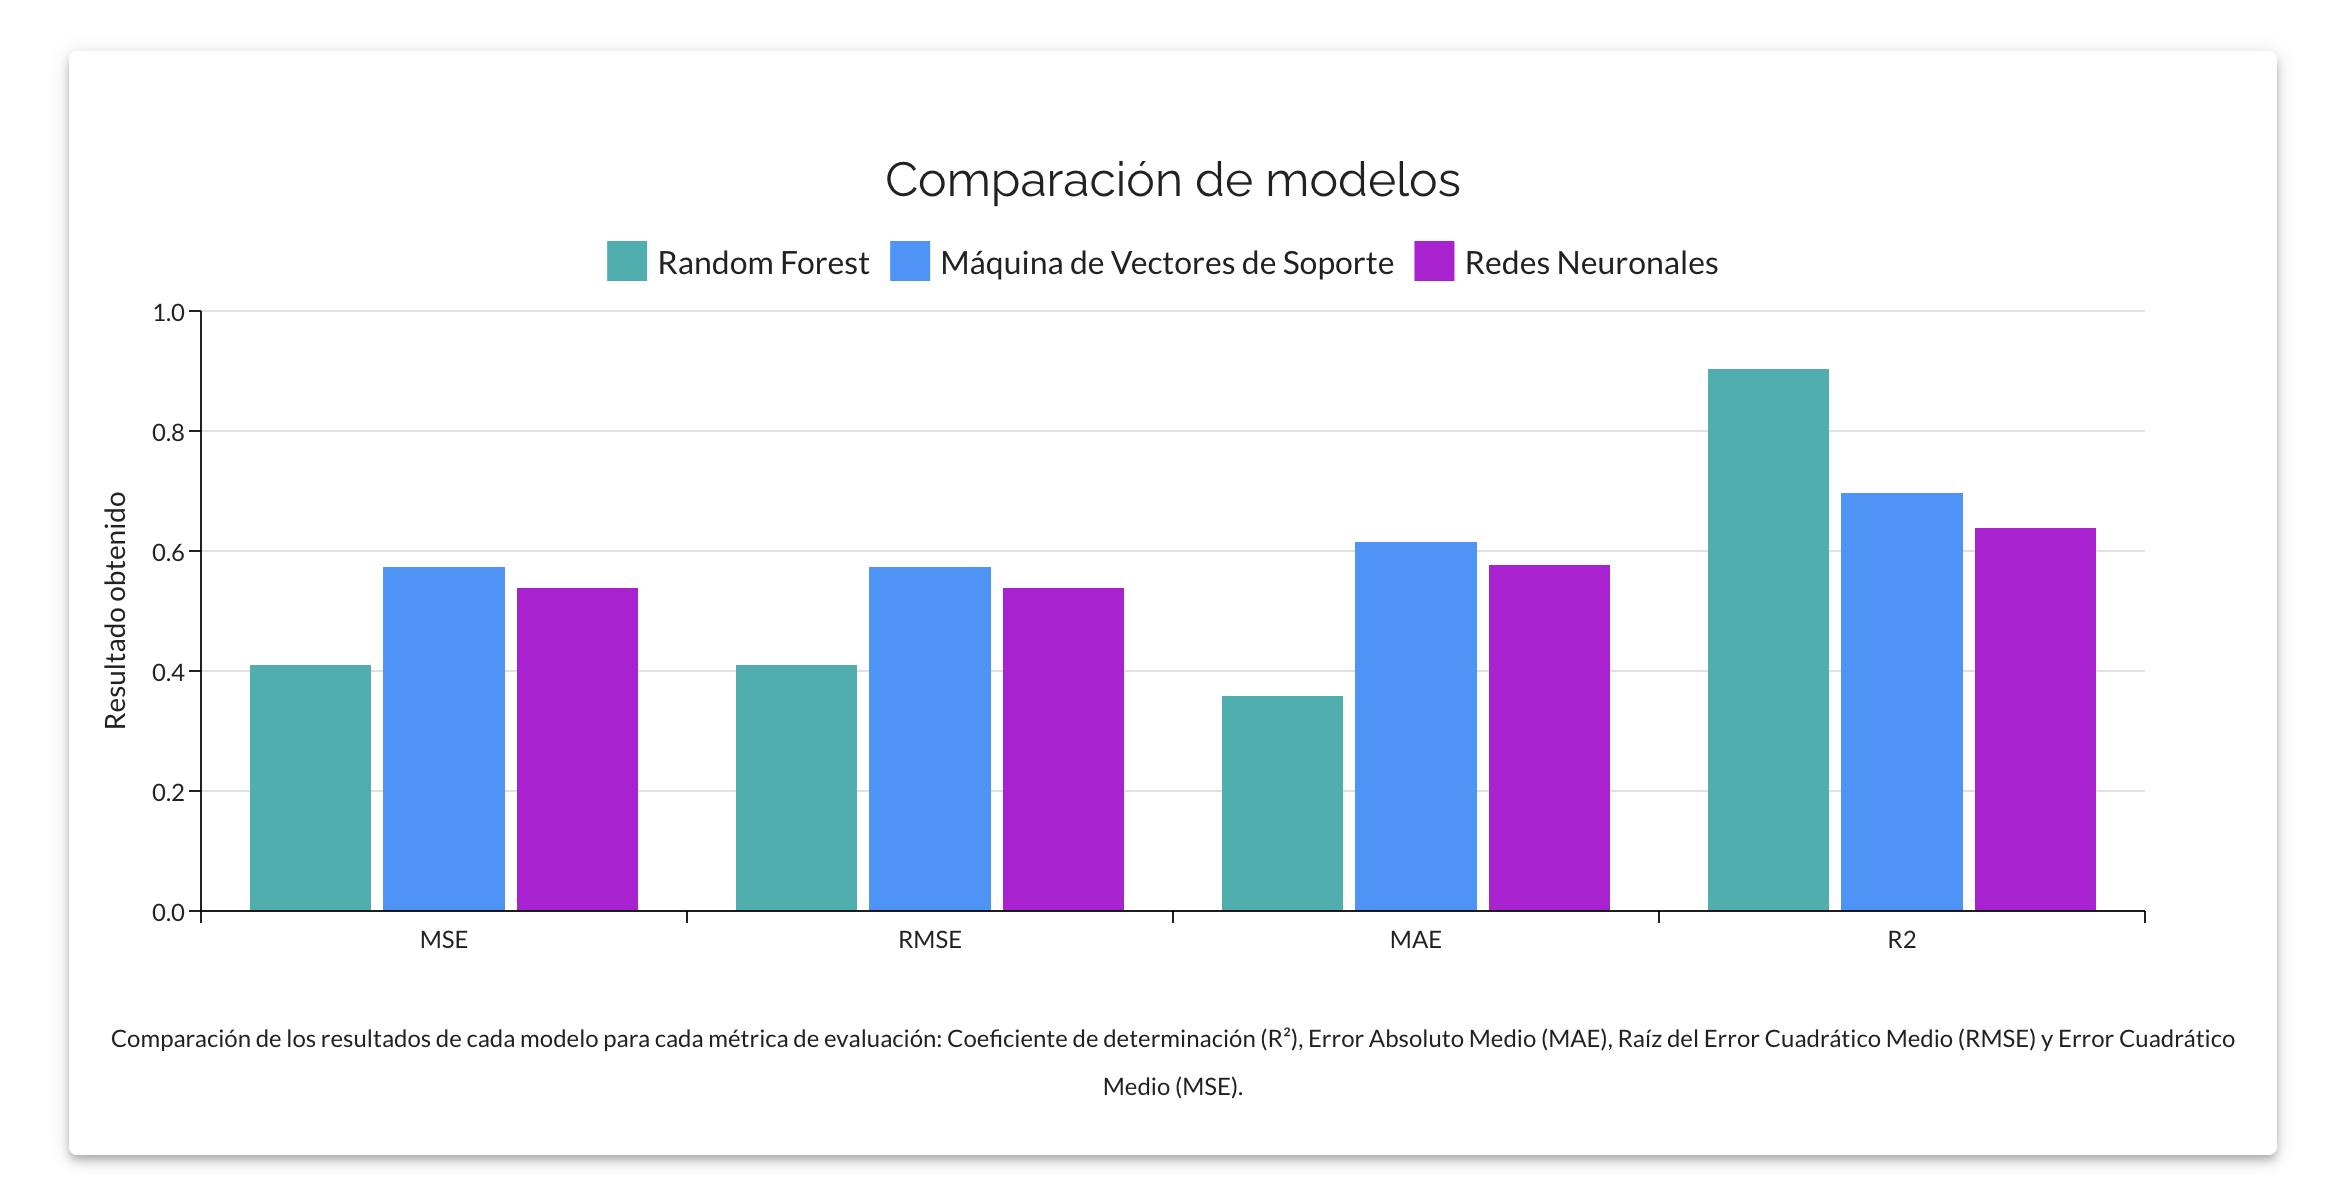
\includegraphics[width=0.8\textwidth]{imagenes/04-acerca-de/graficas-metricas.png}
  \caption{Gráfica de métricas en la página de Acerca de.}
  \label{fig:metricas}
\end{figure}

\section{API Pública}
En esta sección se provee de una breve explicación de la API pública, así como
enlaces a la documentación de la misma. En la figura \ref{fig:api} se muestra la
sección en cuestión en la página.

\begin{figure}[H]
  \centering
  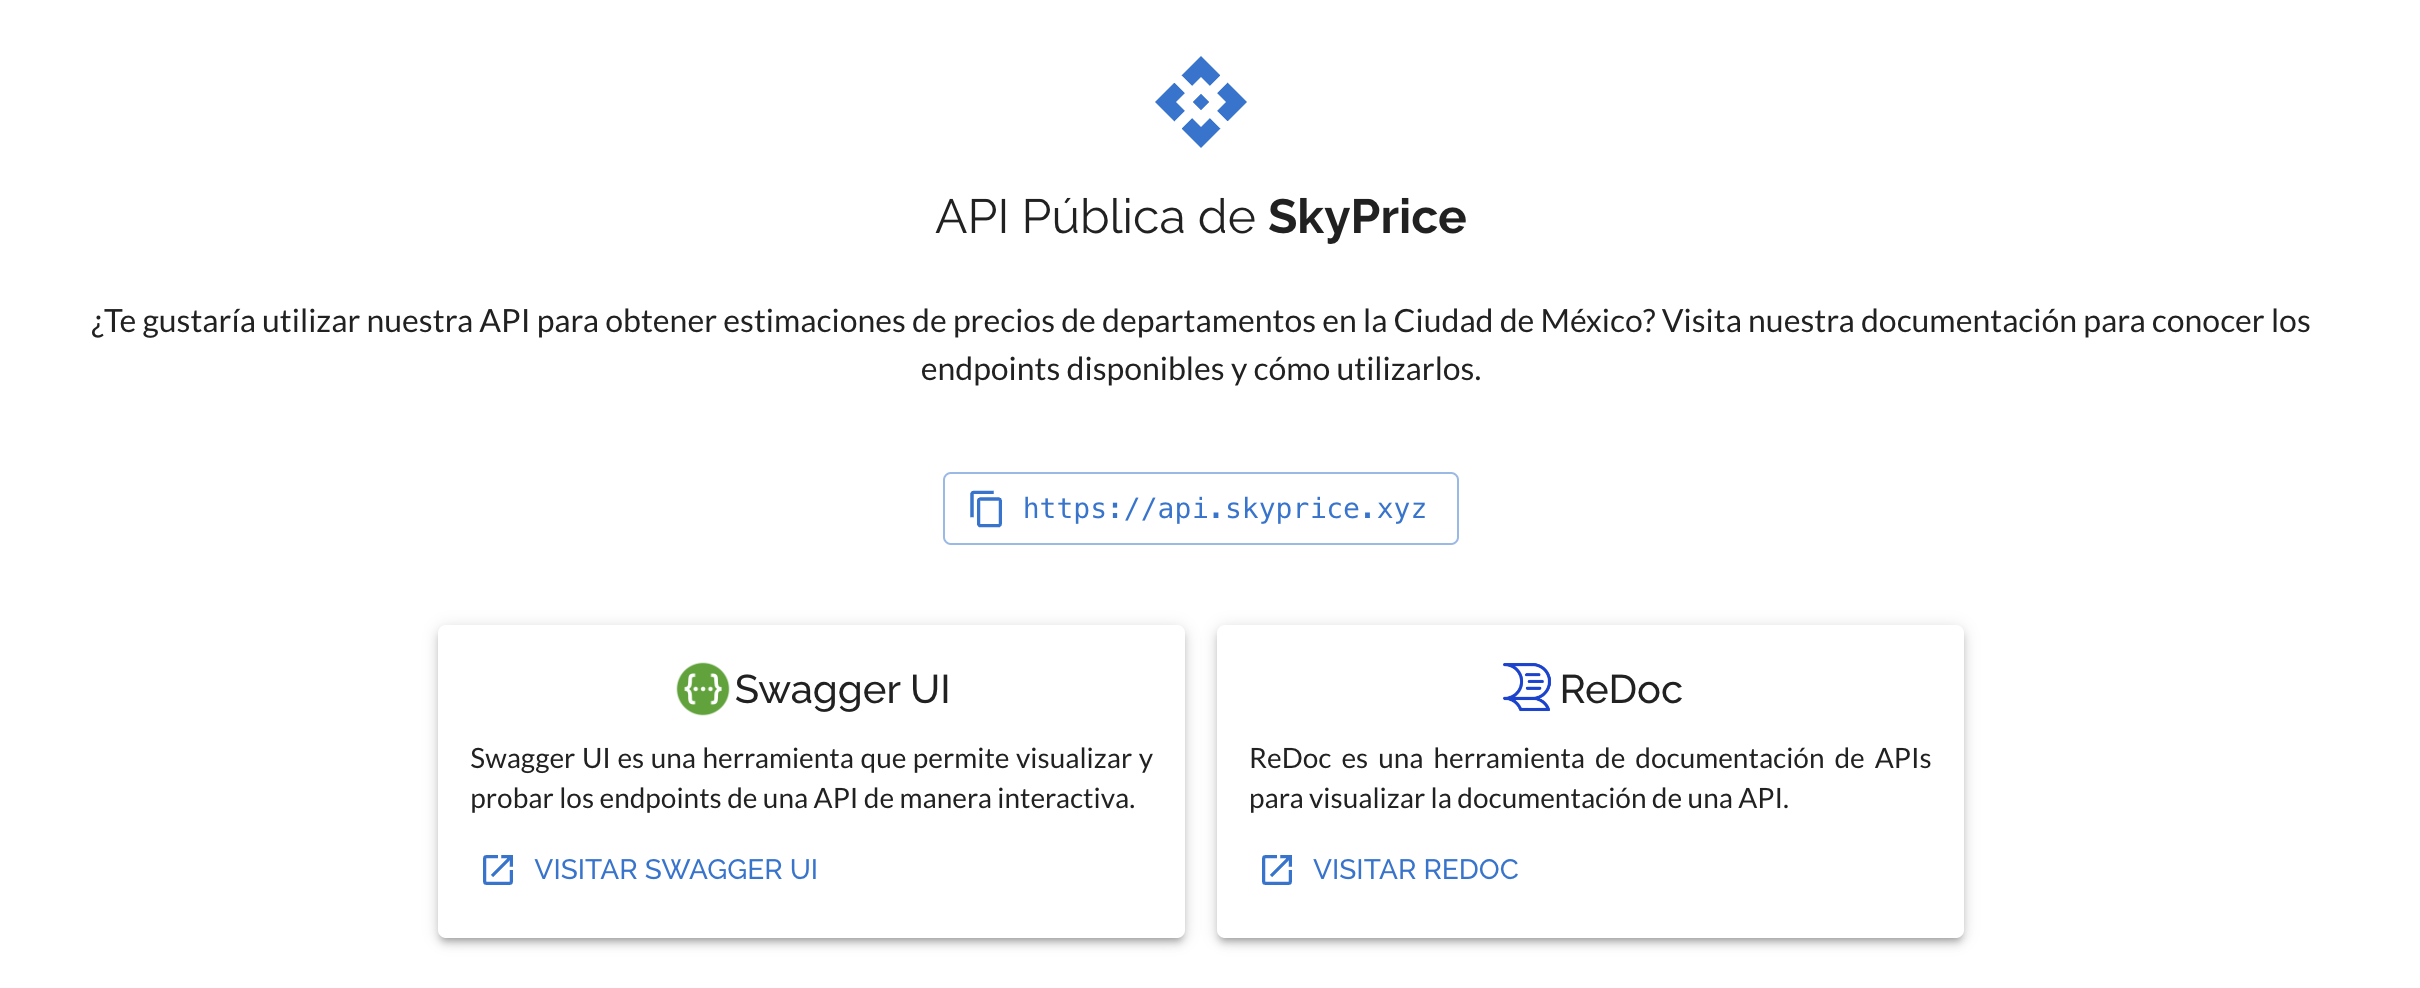
\includegraphics[width=0.8\textwidth]{imagenes/04-acerca-de/api-publica.png}
  \caption{Sección de API pública en la página de Acerca de.}
  \label{fig:api}
\end{figure}

\section{Créditos}
En esta sección se presenta el nombre del autor del proyecto, así como la información
del trabajo de titulación. En la figura \ref{fig:creditos} se muestra la sección en cuestión en la página.

\begin{figure}[H]
  \centering
  
\includegraphics[width=0.8\textwidth]{imagenes/04-acerca-de/creditos.png}
  \caption{Sección de créditos en la página de Acerca de.}
  \label{fig:creditos}
\end{figure}
